\subsection{MIC Architecture}

From the perspective of a developer, it is important to know features of MIC architecture if you want to optimize your applications so that it can run efficiently on Intel Xeon Phi. As your can see in figure \ref{fig:arch} \cite{phibook}, all processors and memory controllers are connected to a Core Ring Interconnect (CRI). Moreover, KNC has NUMA (non-uniform memory access) architecture which means that not all processors have equal access time to all memories.

\begin{figure}[h]
\centering
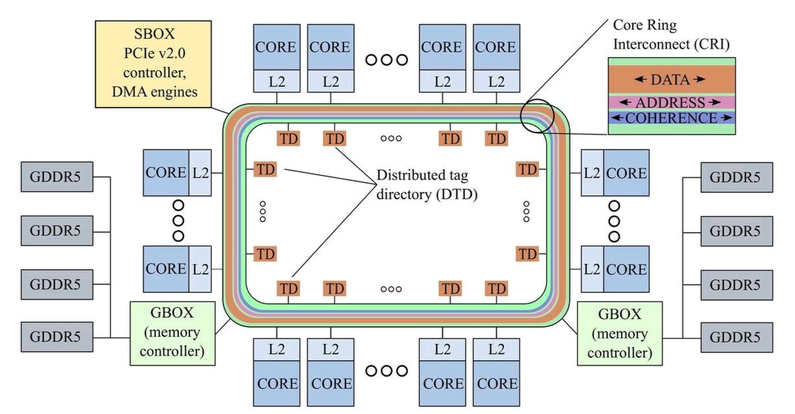
\includegraphics[scale=0.45]{img/mic-arch.png}
\caption{Knights Corner Architecture}
\label{fig:arch}
\end{figure}

KNC is equiped with 61 cores, each core can launch up to 4 hardware threads run in round-robin order. Vector unit, presents in each core, has 512-bit wide registers (vector registers). This functionality allows SIMD operations on up to 16 single precision floating-point numbers, or up to 8 double precision numbers. In terms of memory, KNC has a two-level cache hierarchy (cache level 1 32KB, level 2 512KB) for each core and from 6GB to 16GB shared memory depending on product series. Furthermore,GDDR5 memory can provide a bandwidth of 325GB/s per coprocessor. Of all hardware specifications mentioned above, theoretical peak peformance of KNC is 1200 GFLOPS for double precision and 2400 GFLOPS for single precision.

\subsection{PyMIC}

For several recent years, Python has emerged as a popular scripting language in HPC thanks to its elegance, ease-to-program and ability to reduce development time and make flexible software. However, its convenience trades off for its performance in comparison in C which is a traditional language used in HPC. In 2012, Intel brought to the market a coprocess named Intel Xeon Phi with powerful computing ability and energy-efficient feature, but it only supports C/C++ and Fortran language. Therefore, the creation of PyMIC [ ] has helped to connect C code and Python code so that users can write Python application executed on Intel Xeon Phi (figure \ref{fig:pymic-feat}). To be specific,  PyMIC provides its API to invoke functions (also called kernels) written in C to execute on Intel Xeon Phi. Moreover, PyMIC is not only designed to be a bridge between two languages, its API is also compatable to Numpy, which is Python-API library for scientific computing. Data structures of Numpy can work with PyMIC without causing any conflict.

\begin{figure}[h]
\centering
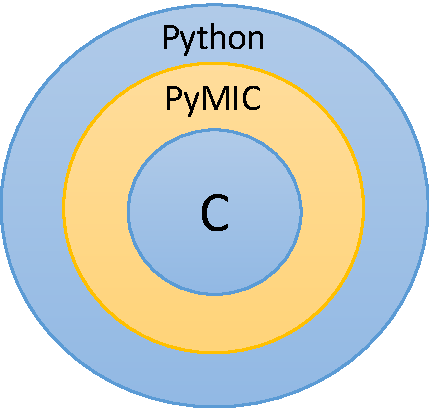
\includegraphics[scale=0.5]{img/pymic-feat.pdf}
\caption{PyMIC functionality}
\label{fig:pymic-feat}
\end{figure}

To provide an easy-to-use interface with slow overhead and full control over data transfering and offloading. Layered architecture of PyMIC is depicted in figure \ref{fig:pymic-arch}. In the lowest layer, Intel Language Extension for Offloading (Intel LEO) is responsible for directly interacting with coprocesser through compiler pragmas or directives. In the higher layer, \_pyMICimpl is a Python extension module written in C/C++, and works as a connector between the highest layer (pyMIC) and the lowest one. To call C functions from pyMIC layer, \_pyMICimpl uses Cython merchanism. Besides, the key class of PyMIC is PyMIC also contains offload\_array class which is totally compatable with class ndarray of Numpy, and several standard kernel that implement array operations.		

\begin{figure}[h]
\centering
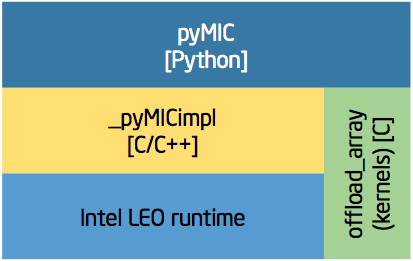
\includegraphics[scale=0.5]{img/pymic-arch.png}
\caption{Architecture of the pyMIC module}
\label{fig:pymic-arch}
\end{figure}

To better understand how PyMIC works, we consider the following example. In figure \ref{fig : Pymic dgemm }, first of all to use PyMIC in Python code, we import package \textbf{pymic}. PyMIC has  In line 5, Xeon Phi card 0 is selected through a global varible \textbf{device} to manage all Xeon Phi cards in a node. In the next line, a \textbf{stream} from that device is created, it functions as a queue to receive requests from host CPU. Kernel \textbf{mydgemm} written in C (figure \ref{fig : C dgemm}) will be compile by C compilier (can be Intel compliler or gcc) into a shared library \textbf{libdgemm.so}, it then is offfloaded to device by Python API, which is described in line 7. In this example, we demonstrate a general matrix multiplication invoked from Python code. Input matrices are initialized  with random values by random function in Numpy package, while output matrix is filled with 0s. However, to do this operation on Xeon Phi, we first have to transfer data to coprocessor. From line 20 to 22, input arrays \textbf{a} and \textbf{b} are transfer to device by enqueueing a request to \textbf{stream}. To be specific, a region of memory will be allocated and data will be copied from host to device. However, with output array \textbf{c}, we do not need to copy data to device by specifiying \textbf{update\_device=False}. Transfering data between host and device is very costly; therefore, to achieve better performance, minimizing data movement is necessary. After transfering data to coprocessor, a computing kernel will be invoked by PyMIC API in line 25 and 26. In order to transfer data back to host CPU, member function \textbf{update\_host()} of \textbf{offload\_array} object will be called. In addtion, all of funtions related to data transfering and array manipulation are done completely asynchronously in chronological order of requests put in queue \textbf{stream}. Using \textbf{sync()} function  of \textbf{stream} in line 28 to wait until the queue is empty. In summary, figure \ref{fig:working mechanism} will gives you an overview of how PyMIC works.

\begin{figure}
    \centering
    \begin{lstlisting}
1  import pymic
2  import numpy as np
3
4  # select device and load kernel library
5  device = pymic.devices[0]
6  stream = device.get_default_stream()
7  library = device.load_library("libdgemm.so")
8
9  # size of the matrices
10 m, n, k = 4096, 4096, 4096
11
12 # create some input data
13 alpha = 1.0
14 beta = 0.0
15 a = np.random.random(m, k) 
16 b = np.random.random(k, n) 
17 c = np.zeros(m, n)
18
19 # create offloaded arrays
20 offl_a = stream.bind(a)
21 offl_b = stream.bind(b)
22 offl_c = stream.bind(c, update_device=False)
23
24 # perform the offload and wait for completion
25 stream.invoke(library.mydgemm,
26                  offl_a, offl_b, offl_c, m, n, k, alpha, beta)
27 offl_a.update_host()
28 stream.sync()
\end{lstlisting}
    \caption{PyMIC Python code example}  
    \label{fig : Pymic dgemm }
\end{figure}

\begin{figure}
    \centering
    \begin{lstlisting}[language=C++]
1  #include <pymic_kernel.h>
2  #include <mkl.h>
3
4  PYMIC_KERNEL
5  void mydgemm(const double *A, const double *B,
6               double *C,
7               const int64_t *m, const int64_t *n,
8               const int64_t *k,
9               const double *alpha,
10              const double *beta) {
11      /* invoke dgemm of MKL's cblas wrapper */
12     cblas_dgemm(CblasRowMajor, CblasNoTrans,
13                  CblasNoTrans,
14                  *m, *n, *k, *alpha, A,
15                  *k, B, *n, *beta, C, *n);
16 }
\end{lstlisting}
    \caption{PyMIC C code example}
    \label{fig : C dgemm}

\end{figure}

\begin{figure}[h]
\centering
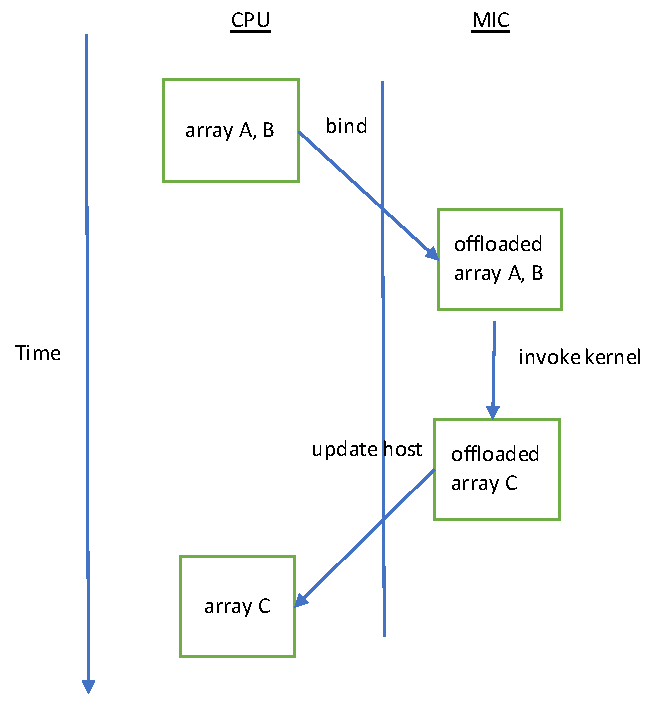
\includegraphics[scale=0.5]{img/working-mechanism.pdf}
\caption{PyMIC working mechanism}
\label{fig:working mechanism}
\end{figure}